\documentclass[acmsmall,screen,review,anonymous,nonacm]{acmart}

%% Written against the frozen tag era6-campaign-3. Every number in it
%% is read from the tree at that state; README.md in this directory
%% names the file each number came from. Target: PLDI 2027 (acmsmall,
%% single column, double-blind: no author names, no funding, no system
%% name that identifies the authors, the project's earlier paper cited
%% in the third person; at most 20 pages of text excluding the
%% bibliography, no appendix in the main file).
%%
%% Preamble from scratch on purpose; this document shares only
%% ../references.bib with the other papers in this directory.
%%
%% TODO author, before submission: (1) Confirm every sentence of the
%% paragraph "Provenance" in sections/intro.tex. It is the paper's
%% disclosure of generative AI — the tool by name and how it was
%% used, as ACM's Policy on Authorship requires — placed in the
%% introduction and made part of the argument, as the project's
%% earlier paper did, rather than in the acknowledgements, which
%% acmart hides under `anonymous`. PLDI 2027's call for papers had no
%% text on the matter on 2026-10-05; if it asks for a statement in a
%% fixed place, repeat it there. (2) Confirm the paragraph "The
%% generator" in sections/registry.tex. (3) The system is unnamed
%% here on purpose; if it is to carry a name in review, it must not
%% be the public one.

\settopmatter{printfolios=true,printccs=false,printacmref=false}

\usepackage{booktabs}
\usepackage{xspace}
\usepackage{tikz}
\usetikzlibrary{positioning,arrows.meta,calc,shapes.geometric}
\usepackage[capitalise,nameinlink]{cleveref}

\newcommand{\code}[1]{\texttt{#1}}
\newcommand{\grade}[1]{\textit{#1}}
\newcommand{\lam}{\Lambda}

\emergencystretch=1.5em
\hyphenation{re-grade re-graded re-grades}

\begin{document}

\title{Judged Whole}
\subtitle{One Gate for Untrusted Verification Infrastructure}

\author{Anonymous Author(s)}
\affiliation{\institution{Anonymous Institution}\country{}}

\begin{abstract}
Verification infrastructure written by a language model cannot be
trusted by construction, and neither can a proof it emits. We
describe a system in which that is not a problem to be solved but the
premise of the design. Every executable --- interpreters, translators
between languages, searches for evidence, certificate checkers, the
maps that carry evidence home --- is generated text, and none of it
is believed: each enters through one gate that runs it against its
own shipped cases and its own shipped mutants, and each result is
graded by \emph{where along its route the evidence was judged}. A
witness is judged by replaying it through the interpreter of the
language the question lives in; a certificate by re-checking it with
that language's checker; a claim with nothing behind it is judged by
nothing and says so. The grade is a distance --- certified at gap
zero, checked one or more translations away, claimed when no judgment
ever ran --- and what a result still rests on, its residual, is
computed from the log by removing everything upstream of the last
judgment. The trusted base is exactly the admitted judges; the kernel
that runs the gate stands outside it and is proved where it is
mathematics, falsified where it is operation, and doubled by a
clean-room second implementation that must agree byte for byte.

We measure the design at one frozen commit, and we measure it against
faults nobody shipped. Of 1,672 sampled source mutants of the
generated translators, carry-backs, and searches, forced past the
gate and played on questions whose answers are known, 16,720 plays
produce 133 wrong answers --- 127 graded claimed, 6 graded checked,
\emph{none} certified --- and every wrong answer's residual names the
faulty component. Of 700 mutants of the seven judges, the gate
refuses half; a differential probe of the survivors finds six real
soundness holes, and revisions that add only test vectors, each
expected value confirmed by an outside tool that never enters the
system, close them. On four benchmarks pinned from HWMCC'24 and
SV-COMP 2025 the system settles 45 of 74, 26 of 79, 47 of 80, and 12
of 55 questions, 49 universal answers resting on a home judge alone;
the generated searches are not competitive with the solvers of those
competitions, and the paper reports the negatives as results.
\end{abstract}

\maketitle

%% §1 — the problem, the sentence, the design in brief, the kernel,
%% the measurements, contributions, and what is not claimed. Written
%% against tag era6-campaign-3; vocabulary is KERNEL.md §12's.

\section{Introduction}
\label{sec:intro}

Verification infrastructure is now being written by language models:
interpreters for the formats benchmarks arrive in, translators between
them, invariant generators, proof scripts, and the checkers that are
supposed to catch the rest. Each such artifact is text produced by a
process that cannot be inspected and that is wrong at an unknown rate,
and the question every deployment faces is what a result computed by
such artifacts is worth. Two answers are current. One verifies the
artifact: repair the proof until a checker accepts it, or generate
the code together with a specification and a proof
\citep{first2023baldur,sun2024clover}. The other distrusts the
artifact and checks its outputs: certifying algorithms
\citep{mcconnell2011certifying}, proof-carrying code
\citep{necula1997pcc}, validated verification witnesses
\citep{beyer2015witnesses}. Both answers are about one artifact at a
time. Neither says what happens when the checker is generated too,
when the translation that carried the program to the checker is
generated, when the map that carries the checker's verdict back to
the original program is generated, and when the search that produced
the evidence was generated last week by the same process.

This paper describes a system built on the premise that every one of
those pieces is untrusted, and judged whole --- and built that way in
fact, not as a thought experiment. It started from an empty
repository with a specification and nothing else, and everything that
has entered since --- every interpreter, translator, search, checker,
and carry-back --- is Python written by a language model and admitted
through one gate. No human wrote any of it, and no human vouches for
it line by line; what stands in for that is the subject of the paper.
The separation that organizes it is a single sentence:

\begin{quote}
\textbf{Generation produces syntax; only interpretation produces
truth.}
\end{quote}

A \emph{language} is a syntax with an \emph{interpreter} --- the
program that runs its programs and reports named observables --- and,
where the language declares \emph{certificate forms}, a
\emph{checker} for each. Interpreters and checkers are the
\emph{judges}, and the trusted base of the system is exactly the set
of admitted judges, a list the kernel prints. Every other executable
is a \emph{transport}: a \emph{translator} from one language to
another, a \emph{carry-back} that brings evidence found at the target
home to the source, or a \emph{search} that looks for evidence --- a
\emph{witness} or a \emph{certificate} --- within a budget. A
transport is untrusted whatever it computes; its output is only ever
as good as the judgment it survives. \textbf{Searches do not decide;
they write. Judges decide.}

The consequence for a result is that its \emph{grade} is geometry. A
question lives at a language; a \emph{route} carries it across
\emph{pairs} of languages to a search; whatever comes back is judged
where it lands, and the \emph{gap} of a result is the number of hops
between the question and the last judgment its evidence passed. Gap
zero is \grade{certified}: a witness replayed by the interpreter of
the language the question lives in, or a certificate discharged by
that language's checker. A positive gap is \grade{checked}: the
certificate was discharged one or more hops away, and the result
still rests on the translators between. No judgment at all is
\grade{claimed}. The \emph{residual} of a result --- what it still
rests on --- is computed from the log as the lineages of the hops
inside the gap plus the judge that ran; every judgment removes
everything upstream of it, so at gap zero the search that found the
evidence, and the route it travelled, are not in the residual at all
(\cref{thm:residual}, proved in Lean).

A design like this makes two claims that can be wrong. The first is
about transports: a faulty translator, carry-back, or search can cost
answers but can never forge a \grade{certified} one, and whatever it
does corrupt says so in its grade and names it in its residual. The
second is about judges: the trusted base is small enough, and tested
well enough, to be believed. We test both by fault injection
(\cref{sec:faults}). For the first we mutate every transport in the
registry, \emph{remove the gate}, force each mutant in, and play it
on questions whose answer is known: 16,720 plays of 1,672 mutants
yield 133 wrong answers, 127 of them \grade{claimed}, 6
\grade{checked} at gap one, and none \grade{certified}; all 133 carry
the faulty entry's lineage in their residual, and seven of the
mutants that answered wrongly had passed the gate. For the second we
mutate the judges and let the gate, and everything admitted
downstream of a judge, try to refuse them: half of 700 are refused,
the survivors concentrate in the certificate checkers, and a
differential probe finds six of them laxer than the checker they
mutate --- real holes in the trusted base. We close the holes without
touching a judge, by revisions that add test vectors whose expected
values are confirmed by tools that never enter the system: a model
checker, a compiler, and the formal model of an instruction set.

The system's own boards are the third measurement
(\cref{sec:boards}). Two domains have entered: hardware, whose root
language is BTOR2 \citep{niemetz2018btor2}, and software, whose root
is a fragment of C; RISC-V is a third language, anchored by no domain
and corroborated by the pairs on either side of it. Four generated
pairs connect the three languages, six generated searches live at
BTOR2 and C, and four benchmarks pinned from HWMCC'24 and SV-COMP
2025 stand at 45 of 74, 26 of 79, 47 of 80, and 12 of 55 questions
settled, with 49 universal answers \grade{certified} at gap zero and
no contradiction. The generated searches are not competitive with the
solvers whose verdicts sit beside the boards, a translation of
hardware into C returned a partial on every route it opened, and ten
times the clock bought one question; the paper reports these because
the system cannot say otherwise.

\paragraph{Provenance}
The premise applies to this paper as well. All of the system --- the
kernel, its tests, the second lineage of its pure half, the Lean
development, every entry in the registry --- and the instruments of
\cref{sec:measurements} --- the fault-injection harness, the
generators of test-vector expectations --- are code generated by
language-model agents (Anthropic's Claude Fable, through the Claude
Code command-line agent). Most of this paper's text, its tables, and
its figures are generated by the same agents, from the specification
and the measurement records. No human reviewed the code or the text
for semantic correctness. The human contribution is the
architecture: the separation of judges from transports, the gate, the
decision that grades are computed and never asserted, and the choices
of what to build, what to measure, and what to claim. What the reader
is offered in place of trust in the writers is what the system offers
in place of trust in its transports. No number here originates with
a model: each is read from logs and stamps the kernel wrote, the
boards regenerate from those logs byte for byte, the fault-injection
counts are recomputed from the deposited records by one command, the
proofs are checked by Lean and their axiom audit is printed at every
build, and the test vectors' expected values were confirmed by tools
that are not generative. The reader need not trust
the writers, human or otherwise, beyond what the thesis itself
requires.

\paragraph{Contributions}
\begin{itemize}
\item A design in which every executable of a verification system is
  untrusted generated text and one gate admits all of them: two
  kinds (language, transport), three judgments an artifact faces on
  crossing a pair (the square, replay, discharge), and two crossings
  nothing judges (\cref{sec:design}).
\item Grades as geometry: gap, grade, and residual computed from the
  log, with the order on results and the residual's properties proved
  (\cref{sec:grades,sec:kernel}).
\item A kernel outside the gate made solid four ways --- proof,
  tests, a clean-room second lineage, content pins --- each worded no
  stronger than what it verifies (\cref{sec:kernel}).
\item A fault-injection method for such systems, and its results: the
  no-forge claim tested with the gate removed, the trusted base's
  exposure measured and localized, six holes found and closed by
  vector-only revisions with outside ground truth (\cref{sec:faults}).
\item Measurements at one frozen commit, every number tied to a file
  in the tree, the negatives reported as results
  (\cref{sec:boards}).
\end{itemize}

\paragraph{What is not claimed}
The square is checked empirically, per program, on a pair's corpus;
per-program translation correctness is not proved. The seal around
generated executables is a blank \code{PATH} and an emptied
environment, measured by tests, and not claimed to be a proof. Half
the sampled judge mutants survive admission; for most of them we can
say only that no certificate we could find distinguishes them from
the judge. The \emph{corroborated} flag has fired only between two
searches, never between two judges. And the boards are not compared
to any solver's on a shared clock; the competitions' verdicts are
recorded beside each question as testimony, never ranked.

%% §2 — one question, two routes: README.md's story in KERNEL.md's
%% words, with the square as the first figure.

\section{One question, two routes}
\label{sec:overview}

Everything the kernel does can be told as the story of one question.
Suppose a benchmark pins a C program $p$ --- a loop over values read
from the outside world, an assertion inside --- and asks: can the
assertion fail within twenty steps? In this generation that sentence
is already formal. C is a \emph{language}: a deterministic syntax
plus a generated, deterministic interpreter $I_C$ exposing named
\emph{observables} --- here \code{bad}, whether an assertion failed,
and \code{depth}, how many statements have run --- and the
certificate forms it can judge, each with a generated checker. The
\emph{question} is $p$, at C, with its \emph{ask}: the observable
\code{bad}, the mode \code{exists}, the bound 20. It lives at C, and
every grade it will ever receive is a distance from that home. The
benchmark enters as a \emph{domain}: a \emph{root} language, the one
its programs are written in, together with its \emph{anchors} ---
labels, supplied vectors, the recorded testimony of outside tools ---
the ungenerable half, and all that entering a new domain costs.

\paragraph{Route one: C to BTOR2}
No search reasons about C directly; the model-checking searches live
at BTOR2, a language of bit-vector machines. What connects the two is
a \emph{pair}: one correspondence, written down as generated code ---
a translator $T$ that turns the elaborated control flow of $p$ into a
machine, one statement one transition, \code{bad} a predicate on
machine state, and \emph{carry-backs} $\lam$ for whatever will need
to come home. Three kinds of artifact cross a pair, and each is
judged on arrival by an interpreter run. The program crosses forward,
and its judgment is \emph{the square} (\cref{fig:square}), closed for
every program of the pair's \emph{corpus} --- the programs it ships
as its own controls --- by running both interpreters:
$I_s(p) \equiv_\pi \lam(I_t(T(p)))$ on the kept observables $\pi$.
The horizontal arrows are untrusted syntax; the vertical arrows are
the judges; nothing horizontal is believed until something vertical
has run. A wrong translator --- buggy, lazy, adversarial --- does not
produce wrong results; it loses squares and is refused at the gate.

%% Figure fig:square, input from the section that discusses it.
\begin{figure}
\centering
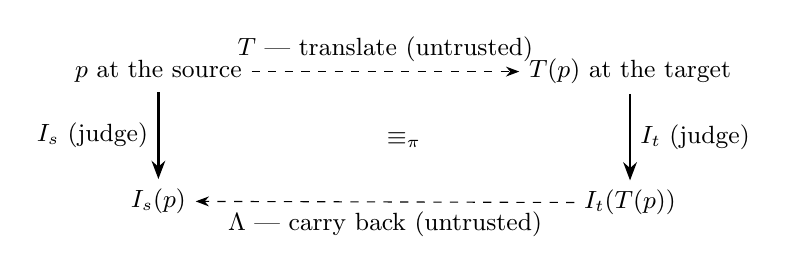
\begin{tikzpicture}[font=\small, >=Stealth, node distance=11mm and 34mm]
  \node (p)  {$p$ at the source};
  \node[right=of p]  (tp) {$T(p)$ at the target};
  \node[below=of p]  (sb) {$I_s(p)$};
  \node[below=of tp] (tb) {$I_t(T(p))$};
  \draw[->, dashed] (p)  -- node[above] {$T$ --- translate (untrusted)} (tp);
  \draw[->, thick] (p)  -- node[left]  {$I_s$ (judge)} (sb);
  \draw[->, thick] (tp) -- node[right] {$I_t$ (judge)} (tb);
  \draw[->, dashed] (tb) -- node[below] {$\lam$ --- carry back (untrusted)} (sb);
  \path (p) -- node[midway] {$\equiv_\pi$} (tb);
\end{tikzpicture}
\Description{A commuting square: the source program is translated
(dashed, untrusted) to the target program; both are interpreted
(solid, judges); the target run is carried back (dashed, untrusted)
and must agree with the source run on the kept observables.}
\caption{The square, the judgment on programs. Dashed arrows are
transports, generated and untrusted; solid arrows are the two
interpreters, the judges. The square is closed empirically, per
corpus program, at admission; the observable renaming $\pi$ is the
projection inside it. Where the translation turns one source frame
into many target frames, a stimulus map and a bound map ride along
and are judged inside the same square against the depths both
interpreters report.}
\label{fig:square}
\end{figure}


\paragraph{At the stop}
The route ends where evidence is written: a \emph{search}, the one
partial transport --- budgeted, allowed to return an honest
\emph{partial} (how far it got, where it failed), and believed by no
one. The searches at BTOR2 are generated solvers: explicit-state
enumeration, bounded model checking, k-induction, IC3. Three kinds of
\emph{evidence} can come back down the route, and each is judged
where it lands. A \emph{witness} --- the failing input sequence ---
is carried back, $\lam$ renaming machine stimuli to the input sites
of $p$, and judged by \emph{replay}: $I_C$ runs $p$ on it where the
question lives. The gap is zero, and gap zero is \grade{certified}.
No generated code can corrupt it: a wrong search, carry-back, or
translator all fail the same way, by not producing a stimulus that
replays. Witnesses need no declared form, because the judge is the
interpreter itself, so a fresh domain certifies existential questions
on the day its root interpreter is admitted. A \emph{bare claim} ---
``no failure within bound $k$'' with nothing behind it --- comes back
unjudged, which is exactly why it cannot raise trust; its grade
floors at \grade{claimed}. A \emph{certificate} --- a k-induction
kernel, a clause invariant --- comes back and is judged by
\emph{discharge}: the checker of the language where it lands
re-checks it. Discharged at BTOR2, the claim grades \grade{checked}
at gap one, and its \emph{residual} is the lineage of the one hop it
has not cleared plus BTOR2's judge, the search no longer among them.
Discharged at C --- once the pair learns to carry the certificate
itself home --- the gap closes and the claim is \grade{certified}.
Each judgment removes everything upstream of it from the residual. If
a replayed witness ever stands beside a covering universal claim,
that is a recorded \emph{contradiction}, never silently resolved: the
witness stands, and the universal's entire chain is marked.

\paragraph{Route two: C to RISC-V to BTOR2}
The same question also travels a longer way: compiled to RISC-V --- a
language whose interpreter is execution of machine code, so reasoning
can happen on the executable when that is the faster place --- then
encoded to BTOR2. Pairs compose into a route; its forward contract is
the componentwise meet --- fragments intersect, kept observables
intersect, bounds cross each hop's bound map --- so a compiler pair
that keeps only \code{bad} makes the whole route a \code{bad}-only
route. What the longer route buys is a different \emph{lineage}: its
generated descent shares nothing with route one, so agreement between
the two would earn the \emph{corroborated} flag, and RISC-V itself,
squeezed by squares against anchored neighbours on both sides, is
corroborated from both directions at once. A \emph{result} is one
play of a route on one question, appended to the run's log with
value, grade, gap, residual, and cost; cost is recorded and never
ranked. Three moves raise performance without touching trust:
\emph{regrade} --- re-discharging a stored certificate closer to home
costs check time, not search time; \emph{hints} --- seeds a pair
passes forward into a search, able to move minutes and not one grade;
and \emph{accelerators} --- a translator or search generated again in
a faster language, admitted only by byte-agreement beside its Python
reference, judges always running the reference.

\paragraph{The loop}
The player --- a language model, or a human at the same command line
--- plays every question along every admitted route, reads the
\emph{frontier} (the questions no result has settled, each with how
far every route got), conjectures the next entry in a fixed order
(new judging and searching first, then new transports, then new
languages), generates it, passes it through the gate, and plays
again, until someone pulls the plug. Pulling the plug is safe at any
moment, because the log is append-only and the best result per
question only ever improves. The rest of this paper makes each word
above exact (\cref{sec:design}), says how the kernel that does this
is itself made trustworthy (\cref{sec:kernel}), lists what has been
admitted (\cref{sec:registry}), and reports what the plays found
(\cref{sec:measurements}).

%% §3 — the design, in lockstep with KERNEL.md §1–§8 and §12; the gap
%% ladder and one loop iteration as figures.

\section{The design}
\label{sec:design}

The specification is written in a vocabulary of fifty words, listed
in its last section, and this section uses no others. The registry holds exactly two
primitive kinds; everything else --- pairs, evidence, grades, routes
--- is derived from them, and the kernel computes with the derived
forms without storing them as kinds.

\subsection{Languages, judges, transports, domains}
\label{sec:kinds}

A \textbf{language} is a deterministic syntax plus a deterministic
interpreter exposing named observables, plus the certificate forms
the language can judge, each shipped with a generated checker.
Interpreters and checkers are the \textbf{judges} --- the system's
only semantic devices --- and the \textbf{trusted base} is exactly
the set of admitted judges: a list the kernel prints, each judge with
the anchors and controls that corroborate it. A \emph{root} is a
language benchmarks arrive in; its interpreter is the trusted floor,
corroborated by the domain's anchors and by nothing generated. Every
other language carries no parent taxonomy. Its interpreter is
corroborated empirically by the squares of the pairs that connect it,
and a language between two anchored neighbours, one square on each
side against a different anchored interpreter, is corroborated from
both sides at once, which no single pair can give.

A \textbf{transport} is a generated function on syntax, declaring its
\emph{fragment} --- the programs it accepts; outside it, a transport
refuses rather than guesses. There are three: the \emph{translator}
$T$, a source program to a target program; the \emph{carry-backs}
$\lam$, a target-side artifact to its source-side form --- a witness
input, a certificate, an observable name; and the \emph{search}, the
one partial transport, given a budget and deterministic for that
budget, allowed to return \emph{partial}. A route ends at exactly one
search. Every transport is untrusted, whatever it computes.

A \textbf{domain} is a root language together with its
\emph{anchors} --- the two things the loop cannot generate for
itself: the format questions arrive in, and the ground truth
(benchmark labels, supplied vectors, the recorded testimony of
outside \emph{oracles}) that corroborates the root's interpreter. A
benchmark lives in exactly one domain, and a domain owns nothing else
and fences nothing: every admitted language, pair, and search serves
every domain, and the gate, not topical relatedness, is the only
membership test.

\subsection{Pairs: the three judgments, and two crossings nothing judges}
\label{sec:pairs}

A \textbf{pair} is the transports that share one correspondence
between a source and a target language --- its translator and its
carry-backs --- declared with a \emph{direction} (exact, over,
under), the observables it \emph{keeps}, the artifacts it carries,
measured cost, its lineage, and its \emph{corpus}, the programs it
ships as its own controls. The grouping is not redundancy: a witness
carried back by one translator's carry-back and replayed against
another translator's output is nonsense; the pair is the statement
that its transports are meaningful together. Three kinds of artifact
move across a pair, and each is judged on arrival by an interpreter
run; there is no other kind of check in the system:

\begin{center}
\small
\begin{tabular}{@{}llll@{}}
\toprule
artifact & moves & transport & judged on arrival by \\
\midrule
a program & forward & \code{T.py} & \textbf{the square}: both interpreters agree on what is kept \\
a witness & back & \code{lam\_wit.py} & \textbf{replay}: the source interpreter runs the program on it \\
a certificate & back & \code{lam\_cert.py} & \textbf{discharge}: the source language's checker re-checks it \\
\bottomrule
\end{tabular}
\end{center}

Two more things cross a pair, and neither is judged. A \textbf{bare
claim} --- ``no failure within bound $k$'' with no certificate behind
it --- crosses back needing no transport, only the pair's observable
renaming and its \emph{bound cap}; nothing judges it, and that is
exactly why it cannot raise trust. A \textbf{hint} --- seeds,
candidates --- crosses forward into a search, trust-inert by
construction: whatever it seeds is judged on arrival, so a hint can
move cost and never a grade.

The square is checked empirically, per corpus program, both
interpreters run at admission; it is not a primitive and not a proof,
and that remains the platform's founding economy. Direction declares
what may cross back --- witnesses along exact and under pairs,
universal objects along exact and over --- and the square is the
empirical evidence for the direction claim. A pair that reifies an
unrolling declares a bound cap: an unbounded object crossing it
arrives as a bound-$k$ fact.

\paragraph{Frames that do not align}
A pair whose translation changes the frame granularity --- one source
frame becoming many target frames, as one machine step becomes a run
of statements --- ships two more transports, judged inside the
square. A \emph{stimulus map} (\code{lam\_in.py}) carries a source
stimulus forward to the one the target interpreter runs on; the
square runs the target side on its output, and the witness carry-back
must be its inverse on the corpus. A \emph{bound map}
(\code{lam\_bound.py}) carries an ask forward and a claim back:
forward, the target depth at which a source firing at frame $t$
lands; back, the largest source frame whose image the claim covers,
or nothing. Neither is trusted: the gate checks the bound map's
structure --- forward strictly monotone with infinity fixed, back its
lower adjoint --- and holds both maps to the depths the two
interpreters report on every corpus stimulus; their mutants must fail
there like any other transport's. The player carries bounds through
every hop, books a claim that ends below the first source frame as a
partial, and never plays a route that revisits a language, so that a
pair in each direction between two languages never plays the round
trip.

Certificate forms belong to languages, not to searches. For a
certificate to come home, what it looks like must be declared where
it lands: a form named at a language and shipped with a generated
checker. A pair's certificate carry-back then maps form to form, per
program, through the correspondence its translator already computes.

\subsection{Evidence: what a search writes}
\label{sec:evidence}

A search is a transport from a language to evidence about its
programs. It declares which observables it can target, it writes, and
it pronounces nothing. A \textbf{witness} is an input; its judge is
the language's own interpreter, by replay, so no generated code
stands between the payload and the trust event. A
\textbf{certificate} is an object of a form the language declares ---
a k-induction kernel, a clause invariant, a box per program point ---
shipped with a checker under the language entry and admitted like
everything else: determinism, example certificates that must
discharge, mutant certificates that must not. Checkers are judges,
part of the trusted base, and deliberately the simplest code in the
system; smallness of judges is the honesty metric. A \textbf{bare
claim} is legal and floors at the lowest grade --- intended selection
pressure: a search that writes checkable certificates outgrades one
that writes bare claims at the same cost, so the ladder itself breeds
certificate printers. A \textbf{partial} --- how far the search got,
where it failed --- is what a route returns when nothing above came
home. A result that decides its question is \emph{settled}: a
replayed witness, or a universal claim covering the asked bound.
A further question mode --- liveness, resource bounds --- is a
new certificate form with a new checker, not a kernel change.

\subsection{Grades are geometry}
\label{sec:grades}

Trust is computed, per result, from where its evidence was judged
(\cref{fig:gap}):
\begin{center}
\small
\begin{tabular}{@{}r@{\ $=$\ }p{0.78\textwidth}@{}}
\textit{gap} & the hops between the question and the last judgment the evidence passed \\
\textit{grade} & \grade{certified} if the gap is 0; \grade{checked} if it is positive; \grade{claimed} if no judgment ever ran \\
\textit{residual} & the lineages of the hops still between the question and that judgment, plus the judge that ran \\
\textit{corroborated} & results of disjoint lineage agree --- an orthogonal flag \\
\end{tabular}
\end{center}
Each judgment removes everything upstream of it from the residual. A
certificate discharged at the search's language removes the search
from what the result rests on --- the search may be garbage; the
checker validated the object. Carried one hop back and discharged
again, it removes that hop too. Discharged where the question lives,
it removes the route entirely: \grade{certified} is
route-independence (\cref{thm:residual}). The fail-safe direction is definitional and
universal: transport is untrusted, so a wrong or adversarial
carry-back can only lose a grade, never forge one. Witnesses have one
property worth stating once: the kernel always replays them where the
question lives, chaining carry-backs across the route, so a witness
is certified or it is not a result at all; an unreplayable witness is
evidence inside a partial, never an answer. A replayed witness is
ground truth, and a covering universal claim beside it is a recorded
\textbf{contradiction}: the witness stands, and the universal's
entire chain --- evidence, judgments, every transport it crossed ---
is marked falsified.

%% Figure fig:gap, input from the section that discusses it.
\begin{figure}
\centering
\resizebox{\textwidth}{!}{%
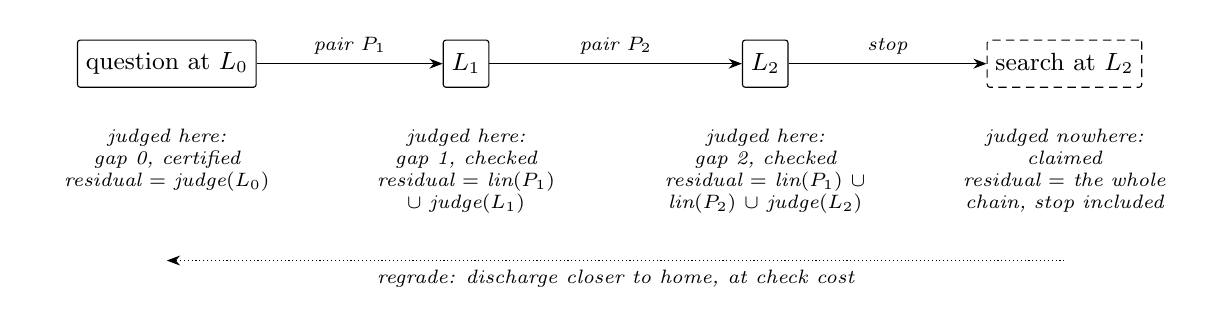
\begin{tikzpicture}[font=\small, >=Stealth,
  hop/.style={draw, rounded corners=1pt, inner sep=3pt, minimum height=6mm},
  lab/.style={font=\scriptsize\itshape, align=center, text width=3.3cm}]
  \node[hop] (q)  at (0,0) {question at $L_0$};
  \node[hop] (l1) at (3.8,0) {$L_1$};
  \node[hop] (l2) at (7.6,0) {$L_2$};
  \node[hop, densely dashed] (s) at (11.4,0) {search at $L_2$};
  \draw[->] (q) -- node[above, font=\scriptsize\itshape] {pair $P_1$} (l1);
  \draw[->] (l1) -- node[above, font=\scriptsize\itshape] {pair $P_2$} (l2);
  \draw[->] (l2) -- node[above, font=\scriptsize\itshape] {stop} (s);
  \node[lab, below=4mm of q]  (g0) {judged here:\\gap 0, \grade{certified}\\residual $=$ judge$(L_0)$};
  \node[lab, below=4mm of l1] (g1) {judged here:\\gap 1, \grade{checked}\\residual $=$ lin$(P_1)$ $\cup$ judge$(L_1)$};
  \node[lab, below=4mm of l2] (g2) {judged here:\\gap 2, \grade{checked}\\residual $=$ lin$(P_1)$ $\cup$ lin$(P_2)$ $\cup$ judge$(L_2)$};
  \node[lab, below=4mm of s]  (g3) {judged nowhere:\\\grade{claimed}\\residual $=$ the whole chain, stop included};
  \draw[->, densely dotted] (11.4,-2.5) -- node[below, font=\scriptsize\itshape] {regrade: discharge closer to home, at check cost} (0,-2.5);
\end{tikzpicture}}
\Description{A route of two pairs from the question's language to
the search's language; under each language the gap and grade a
result judged there receives, and the residual it rests on; a dotted
arrow labelled regrade runs from the search end back to the question.}
\caption{Grades as geometry. A route of two pairs ends at a search;
whatever the search writes is judged where it lands, and the gap
counts the hops between the question and the last judgment. The
residual is the lineage union over the gap segment plus the judge;
every judgment removes everything upstream of it, so at gap 0
nothing but the home judge remains. A bare claim is judged nowhere
and rests on the whole chain. Regrade moves a stored certificate down
this ladder at check cost.}
\label{fig:gap}
\end{figure}


\textbf{Lineage} is a declaration about the descent of generated
procedures. Two judges grown from the same ancestor never corroborate
each other; the corroborated flag requires evidence whose descent
sets are disjoint.

\subsection{Routes, results, the order, the frontier}
\label{sec:routes}

A \textbf{question} is a program, the language it lives in, and its
\emph{ask}: an observable, a mode, and a bound. A \textbf{benchmark}
is a pinned finite set of questions with recorded provenance --- a
sha256 per program, labels where they exist. A \textbf{route} is a
sequence of pairs ending at one search; its forward contract is the
componentwise meet --- fragments intersect, kept observables
intersect, bounds cross each hop's bound map and bound caps take the
minimum, costs add --- and how far an artifact travels back is per
kind: as far as every pair on the way carries it, its grade computed
from where it was last judged, not from what the route promises. A
\textbf{result} is one play of a route on one question, appended to
the log with everything the board needs:
\[
\textit{result} = \{\, \textit{question},\ \textit{route},\
\textit{budget}: \{\textit{caps}, \textit{spent}\},\ \textit{value},\
\textit{grade},\ \textit{gap},\ \textit{residual},\ \textit{lineage} \,\}
\]
where the value is a replayed witness, a universal claim
$\textit{all}(\textit{bound}: k \mid \infty,\ \textit{cert}?)$ graded
by its gap, or a partial with a small typed core the kernel orders on
--- the bound reached --- and free-form progress for the player to
read.

Results order per question by one key, stated in the specification
exactly because the mechanization and the second lineage of the
kernel are both held to it: $(\textit{level}, \textit{bound},
\textit{grade}, \textit{gap})$, compared lexicographically, strictly
greater is better. Level: 0 a partial, 1 a universal claim below the
asked bound, 2 settled. Bound: for a universal claim its bound,
$\infty$ above every number; for a witness, above $\infty$ itself ---
a replayed witness stands above any universal claim on its question;
for a partial the bound it reached. Grade: ungraded below
\grade{claimed} below \grade{checked} below \grade{certified}. Gap: a
smaller gap is better, and ``no check ever ran'' sits below every
finite gap. The incumbent survives only while it is strictly better;
among records of equal key the latest wins, so the board shows the
most recent adjudication of an equally good result. Cost is recorded
in every result and never ranked.

Two performance moves are trust-free because they are judged.
\textbf{Regrade} re-discharges a stored certificate closer to home:
it costs check time, not search time, a shrinking gap is a strictly
improving result under the order, and a revised judge re-derives a
stored certificate's residual the same way, so a proof is always read
under the judges the registry holds now. \textbf{Hints} are forward
artifacts that can move minutes of search and not one grade.

The \textbf{frontier} of a benchmark is the set of questions whose
best result is not settled, each carrying that result and its
progress. The registry and the log are append-only; best-per-question
over an append-only log is monotone: the \emph{ratchet} is a property
of the data structure. Expanding the frontier means strictly
improving some question's best result --- level, bound, grade, or
gap; never cost. The frontier is drawn, not only listed: the
\emph{board} (one row per question, its best result with value,
grade, gap, residual, route, and cost) and the \emph{graph}, both
pure functions of the log, both regenerating byte-identically.

\paragraph{The ledger}
Cost says what a play spent; the ledger says what it bought, in bits
--- profiling, never a grade: the surprisal of a witness under the
uniform measure the interpreter's havoc rule fixes, the log-size of
the stimulus space a bound-$k$ claim exhausts, the compressed length
of a certificate, and per pair an exchange rate measured on its
corpus at admission. A search may ship a trust-inert \code{ledger.py};
what it writes is recorded beside every result.

\subsection{The generation rule: oracles, not organs}
\label{sec:generation}

Every implementation is generated, in Python, and lives as committed
source inside its registry entry. No existing tools: no wrapped
engines, no shelling out, no vendored binaries of someone else's
reasoning. The substrate is the Python interpreter the kernel runs on
and a declared compiler where an accelerator needs building; nothing
that reasons enters except as generated text through the gate. The
rule bounds the system, not the evidence about it. At admission time
a human or the generator may consult an \textbf{oracle} --- an
existing compiler or solver run entirely outside the sealed runner
--- and what the oracle says enters the registry the only way ground
truth ever enters: as anchors with recorded provenance, corroborating
a judge or a transport the way a benchmark label corroborates a root
interpreter. An oracle never enters the trusted base, never runs
inside a play, and its disagreement with a judge is a dispute to
record and adjudicate, never a verdict. The per-question verdicts a
competition archive publishes are anchors of this kind, and so are
the answers of the model checker, the compiler, and the model of an
instruction set that confirmed the test vectors of
\cref{sec:closing}.

Enforcement is layered, and worded no stronger than what each layer
verifies. Statically, there is no manifest field for pointing at a
tool. Dynamically, the runner is sealed: every registered executable
runs in its own process with an environment emptied to a blank
\code{PATH} --- blank rather than absent, because an unset \code{PATH}
is replaced by the platform's default search path, where a tool may
sit --- in a temporary working directory, under a wall cap, and every
check runs twice with byte-compared output. Socially, every
implementation is committed source. The seal makes reaching for a
tool loud and the registry makes it visible; neither is claimed to be
a proof.

\paragraph{Accelerators}
Syntax may accelerate; semantics never does. An entry may ship one
accelerator --- the same implementation generated again in a faster
language --- only for the play-time transports, $T$ and the search,
whose outputs face judges downstream, and it is admitted solely by
byte-agreement with its Python reference on every admission
invocation. Judges always run the reference. The architecture
maximizes the surface where the generator may be wrong for free --- a
wrong translator loses squares, a wrong search loses discharge, a
wrong carry-back loses replay, none can forge --- and the only things
needing care are the judges.

\subsection{The gate}
\label{sec:gate}

Nothing --- no language, pair, search, domain, or any of their
implementations, accelerators included --- enters the system except
by admission, and admission evidence is stamped into the entry by the
gate, never self-reported. One discipline for every kind: determinism
measured (run twice, byte-compare), the checkable relation run on the
entry's own corpus, and two-sided \textbf{controls} --- the intact
implementation must pass and every supplied \textbf{mutant} must
fail, because a checker that cannot be made to fail is unfalsifiable.
Per kind: a language's vectors --- programs with pinned observables
--- interpret as expected, and each shipped checker discharges its
example certificates and refuses its mutant ones; a pair's every
carried artifact round-trips per corpus program --- squares close,
stimuli replay, certificates discharge --- with mutants per artifact
kind; a search's written evidence on its corpus must judge valid, its
negative controls must fail, and its budget determinism must hold; a
domain names its root and every anchor's provenance. An entry that
fails leaves no stamp and no trace in routing.

\paragraph{Revision, not mutation}
An admitted entry is never edited. Every \textbf{stamp} pins the
entry's bytes with a content hash the loader re-verifies, defined in
the specification rather than left to an implementation: over every
regular file under the entry, excluding the top-level manifest,
dotfiles, and bytecode, the map from entry-relative path to the
sha256 of the file's bytes, serialized as JSON with sorted keys,
hashed once more. Extension arrives as a new entry \code{<name>@<r>}
carrying a revision number and its predecessor's hash. The gate for a
revision is the ordinary kind gate plus conservativity: the new
implementation must byte-agree with its predecessor on the
predecessor's whole checkable surface --- its vectors or corpus, and
for a language the corpora of every admitted pair bound to it. A name
binds to its highest admitted revision; predecessors stay in the
tree; results name the revision they ran. Adding a carry-back to an
admitted pair is the intended common case: the old transports are the
conserved surface, the new one is gated fresh.

\subsection{The loop, the conjecture order, bootstrap from empty}
\label{sec:loop}

The player is presented a benchmark and runs until a human pulls the
plug: play --- for every question, run the admitted
routes within budget, the kernel recording results; read the frontier
--- the open questions with their progress, and the grades, since a
board full of \grade{claimed} and \grade{checked} is itself frontier;
conjecture, in the \textbf{conjecture order} --- (a) new judging and
searching for existing languages, (b) new transports, including
carry-backs retrofitted onto admitted pairs by revision and a
translator from a root that reaches no hub to the nearest one, (c)
new languages, proposed only when a translation or solving move keeps
winning ad hoc; generate, gate, register; re-play. Semantics first,
then syntax: new syntax is earned by demonstrated semantics, never
invented ahead of it. The trust story in one sentence: \textbf{the
generator never writes a result; only the kernel does, by running
judges over transported evidence.} 

The kernel ships with zero languages, zero transports, zero domains.
Presented a benchmark, the first admissions are the domain --- root
name plus anchors, the ungenerable half --- then the root language's
interpreter, then a first naive search in pure Python. Witnesses need
no declared form, so existential questions can settle
\grade{certified} with a single admitted interpreter; the first
certificate form and checker arrive when universal questions need
better than \grade{claimed}. \Cref{sec:registry} reports that this
is how the tree was in fact populated.

%% §4 — the kernel made solid four ways, in lockstep with KERNEL.md §9,
%% kernel/mechanization/README.md and the theorem names in
%% Kernel/Key.lean and Kernel/Trust.lean, kernel/tests/__init__.py,
%% and kernel/second/README.md. Line counts: wc -l at the tag.

\section{The kernel, made solid four ways}
\label{sec:kernel}

The kernel is the fixed part: the gate, the sealed runner, the result
order, the registry loader, and the driver that plays, regrades, and
renders --- five stdlib-only Python modules of 2,654 lines at the tag
(\code{driver.py} 689, \code{gate.py} 1,238, \code{registry.py} 191,
\code{results.py} 419, \code{runner.py} 85, and a 32-line package
file). It is the one piece of code the gate cannot judge, because it
is the gate; it is generated like everything else in the tree; and
so four disciplines stand in for the gate, each worded no stronger
than what it verifies.

\paragraph{It computes no truth of its own}
The kernel runs judges, compares bytes, orders results, and draws the
log. A kernel bug can lose a result or misgrade one; the property
that it can never forge one --- no record reaches \grade{certified}
unless an interpreter run where the question lives passed, whatever a
search, a carry-back, or a translator wrote --- is stated in the
specification and falsified by test
(\code{kernel/tests/test\_forge.py}). On a registry bootstrapped from
empty through the real gate --- two toy languages, one pair, one
search, one domain --- a search that prints a witness together with
the words \code{"grade": "certified"} never becomes a result, because
its witness does not replay; a bogus certificate floors at
\grade{claimed}; a bare claim is the checkless crossing; true numbers
on an unsafe program do not discharge; a broken carry-back only loses
the witness; a route missing a carry-back is a partial, never an
answer; an observable the pair does not keep is a partial; and
\code{regrade} lifts a stored proof to \grade{certified} by check
time alone once the pair learns to carry certificates.

\paragraph{The half that is mathematics is proved}
The Lean development under \code{kernel/mechanization/}
\citep{demoura2021lean4} --- 502 lines, no dependencies beyond the
Lean core, toolchain pinned --- proves, for exactly the key of
\cref{sec:routes}, the properties the specification asks for. In
\code{Kernel/Key.lean}: the order is a strict partial order
(\textsf{Key.lt\_irrefl}, \textsf{Key.lt\_trans},
\textsf{Key.lt\_asymm}, axiom-free); best-per-question is monotone
under log append --- the ratchet (\textsf{best\_mono}); once settled,
always settled (\textsf{settled\_ratchet}); at a fixed level and
bound the gap never grows and grades only move up
(\textsf{le\_same\_value}, \textsf{same\_value\_ratchet}), with
\textsf{grade\_moves\_key}, \textsf{gap\_moves\_key}, and
\textsf{first\_check\_moves\_key} saying that a regrade, which keeps
the value, is a strict improvement exactly when it moves the grade or
the gap. In \code{Kernel/Trust.lean} the residual is defined as the
lineage union over the gap segment plus the judge,
$\textit{residual}(\textit{hops}, g, \textit{judge}) =
\bigcup_{i<g} \textit{hops}_i \cup \textit{judge}$, and proved to be
exactly that meet (\textsf{mem\_residual}), from which: gap 0 rests
on the judge alone (\textsf{residual\_gap\_zero}) ---
\grade{certified} is route-independent as a theorem; a smaller gap
never adds trust (\textsf{residual\_mono}); every judgment removes
everything upstream of it
(\textsf{residual\_check\_removes\_upstream}); and the stop is never
in the residual (\textsf{residual\_stop\_free},
\textsf{residual\_le\_whole}) --- once anything checked, the search's
own descent is gone. The build prints the axiom audit for every
theorem: the order lemmas are axiom-free; the fold lemmas rest on
\textsf{propext} and \textsf{Quot.sound} through
\textsf{List.foldl\_append}, and so do the residual lemmas
(\textsf{residual\_gap\_zero} on \textsf{propext} alone). What the model does not cover is said in
its README so the layout never overstates: the proofs are about the
order and the residual as functions of keys and lineages, not about
the Python that computes them --- that correspondence is the job of
\code{test\_order.py}, which runs the same properties against
\code{results.key} on random records --- and the bound is a natural
number under an order-embedding of the Python's stand-ins, which
lexicographic order cannot distinguish from the original.

\paragraph{The half that is operation is falsified}
The test suite (\code{python3 -m kernel.tests}; 2,077 lines in eight
modules and the toy registry) is the gate turned on the kernel.
\code{test\_gate} runs the gate against the registry's own controls:
every bound entry's stamp is re-derived by re-running its admission
--- its agreement counts a floor, since a stamp is never rewritten
and a pair may join after the language it binds to was stamped, an
allowance pinned the first time it was needed --- and every supplied
mutant is refused again; with \code{HG\_SLOW=1} every admitted entry
of every kind is re-gated, old revisions included; and on the toy
registry every way of failing the gate fails it: a language without
controls is unfalsifiable, a mutant that passes means the vectors are
blind, a judge that accepts anything is refused, reaching for a tool
is loud, judges are never accelerated, nondeterminism is refused, a
revision must agree with its predecessor, a translator mutant that
keeps the square is refused, a lying search is refused because its
witness does not replay, a search that only abstains is vacuous, a
verdict against a label is refused. \code{test\_seal} measures the
seal: the environment holds nothing but a blank \code{PATH}, the
working directory is scratch and gone afterwards, no tool can be
found --- not even on the platform default path --- determinism is
measured rather than declared, and a hit wall is a result, not an
exception. A test that found the seal weaker than the specification
claimed --- an unset \code{PATH} still found \code{/usr/bin/python3}
--- is how the blank \code{PATH} got into the specification.
\code{test\_registry} recomputes the content pin from its definition
for every stamp and refuses changed bytes, pinless stamps, and two
entries claiming one name at one revision. \code{test\_misaligned}
exercises the frame contract of \cref{sec:pairs} end to end, mutants
included. \code{test\_regenerate} regenerates the board and the graph
of every pinned run byte-identically from the log.

\paragraph{A second lineage agrees}
\code{kernel/second/} is the kernel's pure half --- registry loading
with pin verification, benchmark pins, the order, best-per-question,
the frontier, contradictions, corroboration, the board, the graph,
the base; 727 lines --- generated clean-room from the specification
and the committed data alone, never from the first kernel's source.
Its README records the protocol: what was read (the specification,
the manifests, the runs, directory listings), what was run (the first
kernel only as a black box through its command line; never
\code{play}, \code{admit}, or \code{regrade}), one disclosure (an
early traceback on a corrupt registry named two source files and
line numbers; the first kernel now refuses a corrupt registry without
a traceback), and where the specification left it guessing --- eleven
listed ambiguities on inputs no pinned run exercises. It is held to
byte-agreement with the first kernel on \code{base}, \code{report},
and \code{graph} over every pinned run and over a synthetic run
holding the corners no pinned run exercises (\code{test\_second}),
and a runtime audit hook on \code{open} confirms that no module of it
reads any file of the first kernel (the import system loads the
bytecode of the \code{kernel} package's own \code{\_\_init\_\_},
because \code{second} is its subpackage, and nothing else). This is the accelerator discipline of \cref{sec:generation}
turned on the kernel: two implementations of disjoint descent that
agree on every byte corroborate each other, as two judges do. Where
they disagreed while being built --- the key's tie rule, the pin's
exclusions, the binding rule for revisions --- the specification was
made to say which is right, and now does.

Manual review is the last discipline, and the four above are what
make it tractable: what must be read is exactly the trusted base ---
the admitted judges, printed by \code{base} (\cref{sec:registry}),
and the kernel's five modules --- and the reviewer reads theorem
statements, tests, and a second implementation's disagreements rather
than a story.

%% §5 — what was admitted, in the order it was admitted: the manifests'
%% notes and stamps under registry/, and `python3 -m kernel.driver base`.

\section{What was admitted}
\label{sec:registry}

Everything under \code{registry/} at the tag entered through the gate
of \cref{sec:gate}, in the order the conjecture order prescribes, and
every entry carries its stamp. \Cref{fig:registry} draws the
registry; \cref{tab:base} is the trusted base as the kernel prints
it.

%% The registry at the tag, drawn: languages, pairs, searches. Names
%% carry their highest admitted revision (registry/*/ directory names).
\begin{figure}
\centering
\resizebox{\textwidth}{!}{%
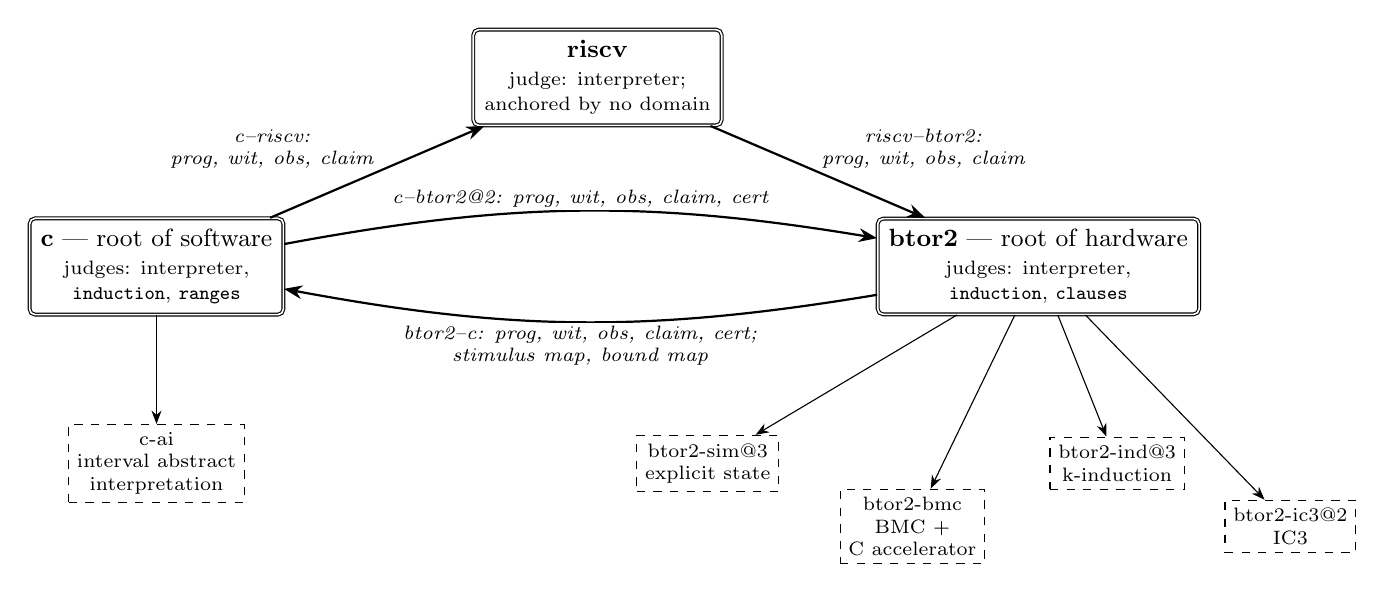
\begin{tikzpicture}[font=\small, >=Stealth,
  lang/.style={draw, double, rounded corners=2pt, inner sep=4pt, align=center},
  srch/.style={draw, dashed, inner sep=3pt, align=center, font=\scriptsize},
  pl/.style={font=\scriptsize\itshape, align=center, fill=white, inner sep=1pt}]
  \node[lang] (c) at (0,0) {\textbf{c} --- root of software\\[-1pt]\scriptsize judges: interpreter,\\[-2pt]\scriptsize \code{induction}, \code{ranges}};
  \node[lang] (r) at (5.6,2.4) {\textbf{riscv}\\[-1pt]\scriptsize judge: interpreter;\\[-2pt]\scriptsize anchored by no domain};
  \node[lang] (b) at (11.2,0) {\textbf{btor2} --- root of hardware\\[-1pt]\scriptsize judges: interpreter,\\[-2pt]\scriptsize \code{induction}, \code{clauses}};
  \draw[->, thick] (c) to[bend left=10] node[pl, above] {c--btor2@2: prog, wit, obs, claim, cert} (b);
  \draw[->, thick] (b) to[bend left=10] node[pl, below] {btor2--c: prog, wit, obs, claim, cert;\\stimulus map, bound map} (c);
  \draw[->, thick] (c) -- node[pl, above left] {c--riscv:\\prog, wit, obs, claim} (r);
  \draw[->, thick] (r) -- node[pl, above right] {riscv--btor2:\\prog, wit, obs, claim} (b);
  \node[srch] (cai) at (0,-2.5) {c-ai\\interval abstract\\interpretation};
  \node[srch] (bs) at (7.0,-2.5) {btor2-sim@3\\explicit state};
  \node[srch] (bb) at (9.6,-3.3) {btor2-bmc\\BMC $+$\\C accelerator};
  \node[srch] (bi) at (12.2,-2.5) {btor2-ind@3\\k-induction};
  \node[srch] (bc) at (14.4,-3.3) {btor2-ic3@2\\IC3};
  \draw[->] (c) -- (cai);
  \draw[->] (b) -- (bs); \draw[->] (b) -- (bb); \draw[->] (b) -- (bi); \draw[->] (b) -- (bc);
\end{tikzpicture}}
\Description{Three language nodes (c, riscv, btor2) with four
arrows for the pairs between them, and five dashed search nodes hanging
from the languages they live at: one at c, four at btor2.}
\caption{The registry at the tag: three languages (double borders),
four pairs (solid arrows, labelled with the artifacts they carry),
five searches (dashed, at the language they live at). Names carry
their highest admitted revision. Every node interprets; every edge
translates; every search writes. Routes never revisit a language, so
the two pairs between \code{c} and \code{btor2} never play the round
trip.}
\label{fig:registry}
\end{figure}


\begin{table}
\caption{The trusted base at the tag, as \code{python3 -m
kernel.driver base} prints it --- judges only; everything else in the
registry is untrusted syntax. Vectors are programs with pinned
observables; controls are mutants the gate refused. For a checker,
vectors are example certificates that must discharge and controls
mutant certificates that must not. Sizes are lines of Python at the
tag.}
\label{tab:base}
\centering
\small
\begin{tabular}{@{}llrrrl@{}}
\toprule
judge & kind & vectors & controls & lines & corroborated by \\
\midrule
\code{btor2@5} & interpreter & 11 & 6 & 390 & hardware (3 anchors) \\
\quad \code{btor2:induction} & checker & 6 & 6 & 1,620 & \\
\quad \code{btor2:clauses} & checker & 4 & 4 & 1,618 & \\
\code{c@5} & interpreter & 12 & 6 & 1,422 & software (3 anchors) \\
\quad \code{c:induction} & checker & 9 & 9 & 4,534 & \\
\quad \code{c:ranges} & checker & 5 & 5 & 3,935 & \\
\code{riscv} & interpreter & 13 & 8 & 603 & no domain; its pairs' squares only \\
\bottomrule
\end{tabular}
\end{table}

\paragraph{The first campaign (2026-08-29 and 30)}
The hardware domain entered first, before its root interpreter
existed: root \code{btor2}, three anchors --- the HWMCC'24 bit-vector
track with the official verdicts of the competing solvers as recorded
testimony, the pinned benchmark, and eleven hand-written machines
with pinned observables. Then the BTOR2 interpreter, the trusted
floor: bit-vectors, the signed division family, arrays, constraints;
corroborated by nothing generated. Then the naive first citizen,
\code{btor2-sim}: exhaustive breadth-first enumeration with fixpoint
detection when the free-input space is small, deterministic guided
sampling otherwise, witnesses only in the second case. Then
\code{btor2-bmc}: bit-blasting per frame to a hash-consed
and-inverter graph, Tseitin encoding, a generated CDCL SAT solver,
every model replayed through the interpreter semantics before it is
emitted; a bare $\textit{all}(k)$ after unsat at every depth up to
$k$; and an accelerator, \code{solve\_fast.c}, mirroring the
reference formula by formula, admitted by byte-agreement on the six
corpus machines. The software domain and the C interpreter followed
--- the preprocessor-free ILP32 integer fragment SV-COMP's loop and
bit-vector tasks are written in, semantics total and deterministic
and chosen to be exactly mirrorable by a bit-vector machine,
validated beyond its twelve vectors by the recorded testimony of
\code{clang -O0 -fwrapv} on random stimuli over the in-fragment
corpus (1,045 verdict agreements, none divergent), the compiler never
entering. Then RISC-V as the middle vertex, anchored by no domain.
Then the three pairs of the triangle --- \code{c--btor2},
\code{c--riscv}, \code{riscv--btor2} --- each carrying programs,
witnesses, observables, and claims, with mutants per artifact kind
(translator mutants that lose squares, carry-back mutants that drop
values or shift frames) and its exchange rate measured: 3.65, 5.37,
and 3.13 target bytes per source byte, as stamped on the revisions
that bind today (the first revision of \code{c--btor2}, on a corpus
of seven programs, measured 3.97). Then two certificate forms on
BTOR2 by revision of the language --- \code{induction}
(bit-invariants, discharged by three one-step SAT queries for init,
consecution, and safety; k-induction, by base and step) and
\code{clauses} (a conjunction of clauses over state bits, as IC3
converges to) --- with the two searches that write them,
\code{btor2-ind} and \code{btor2-ic3}. Then C's own \code{induction}
judge, the certificate carry-back of the C-to-BTOR2 pair by revision
(\code{c--btor2@2}), and a further revision of C's judge that builds
its machine by the RISC-V road --- front end, fenced RV64 blocks,
transition system, sharing no text with the C-to-BTOR2 encoding ---
so that a proof which travelled the C-to-BTOR2 pair is certified by
an encoding that pair never touched. Last, arrays reached the judges:
the bounded checker's eager reduction, with its congruence and
extensionality lemmas, carried into both BTOR2 checkers, C's judge,
and the inductive search.

\paragraph{The reverse edge (2026-09-06 and 07)}
The C hub gained a third certificate form, \code{ranges} --- per
program point a box over the scalar slots in their own types,
unlisted points asserted unreachable, discharged by init,
consecution, and safety on the same machine C's \code{induction}
judge builds --- and its first search, \code{c-ai}: interval abstract
interpretation over the elaborated control-flow graph with exact wrap
images, threshold widening from the program's own constants, and a
narrowing whose every round is accepted only after the recomputed
transformer is verified to stay below it; it writes a \code{ranges}
certificate or an honest partial and never a bare claim. The frame
contract of \cref{sec:pairs} was written into the specification and
its tests into the suite, and on it the pair \code{btor2--c} was
admitted with all five channels: every state, input, and
combinational node a global of the smallest unsigned container
holding its width, masked after every operation; one statement per
node, \code{ite} and every conditional branch-free; a violated
constraint clearing a sticky flag; the states assigned together at
the end of the loop body, so that a \code{bad} at machine frame $t$
is observed at C frame $n_0 + n \cdot t + \textit{bad}$, the three
numbers the translator writes as a header. Its corpus is seventeen
machines --- the six bit-vector vectors of \code{btor2@5}, eight
small machines written for the controls, three from
\code{hwmcc24-mini}; six certificates round-trip (four \code{ranges}
boxes bit-blasted into \code{clauses} over state bits, one
k-induction rescaled, one clause invariant carried bit for bit);
thirteen mutants are refused (four on programs, two on witnesses,
three on certificates, two on the stimulus map, two on the bound
map); its exchange rate is 4.19 bytes per byte. Out of revision 1's
fragment, refused loudly: array sorts, widths above 64, non-constant
initial values.

\paragraph{Revisions}
Eleven language entries, five pair entries, ten search entries, and
two domains stand in the tree at the tag; a name binds to its highest
revision. The revisions tell the campaign's small history without
editing anything. \code{btor2-sim@2} evaluated the signed division
family after four \code{hwmcc24-mini} machines crashed the first
revision and gained a ledger; \code{@3} scaled its effort by model
size after fixed budgets ran past twice the wall on translated C
programs. \code{btor2-ind@2} and \code{btor2-ic3@2} blasted the
signed division family after thirteen \code{svcomp25-mini} programs
and four \code{hwmcc24-mini} programs crashed the first revisions,
and turned every remaining unsupported operation into a partial
instead of a crash; \code{btor2-ind@3} ran on the bounded checker's
array engine. Each was byte-identical to its predecessor on the
predecessor's corpus, which is what lets the stamps that depend on it
keep their meaning.

%% §6 — the measurements, every number read at tag era6-campaign-3
%% from kernel/faults/results/*.jsonl, runs/*/frontier.md,
%% runs/*/log.jsonl, runs/*/benchmark.json (the `official` field),
%% oracles/packs/languages/*/ and the registry stamps. README.md in
%% this directory lists the provenance file by file.

\section{Measurements}
\label{sec:measurements}

Every number in this section is read from the tree at one tag. Three
things are measured: what faults placed deliberately do to the gate
and to the grades (\cref{sec:faults}); what it took to close what
they found (\cref{sec:closing}); and what the system settles on four
pinned benchmarks (\cref{sec:boards}).

\subsection{Fault injection}
\label{sec:faults}

Every entry ships its own mutants and the gate refuses them; that
says the controls can fail, not how much they see. We therefore
mutate the registry ourselves, in the manner of mutation testing
\citep{demillo1978hints,jia2011mutation}. A \emph{mutant} is one
executable with one classical fault: a comparison or an arithmetic or
bitwise operator replaced, \code{and} and \code{or} exchanged, a
negation dropped, a branch condition negated, an integer constant
moved by one or a truth constant flipped, or a statement with no
binding effect removed. Sites are enumerated over the syntax tree of
every executable a name binds to --- the seven judges and the
eighteen transports (twelve translators, carry-backs, and maps of the
four pairs; six searches) --- and one hundred per file are drawn by a
hash of the site, so the sample is reproducible; two small files have
fewer sites, giving 700 judge mutants and 1,672 transport mutants. A
mutant is staged in a scratch copy of its entry and run sealed like
everything else, under a wall of four times the intact entry's
longest run and a memory cap; the registry and the logs are never
written. Each experiment first runs the intact file and its
unparsed-and-reparsed identity, which must behave as the entry does.

\paragraph{At the gate}
A mutated entry faces what an entry of its kind faces at admission,
in order, and the first refusal is recorded: its \emph{own} vectors,
corpus, and controls; \emph{conservativity}, byte-agreement with its
predecessor on the predecessor's checkable surface; and, for a judge
only, its \emph{dependents} --- the admission of every pair and
search that runs the judge, re-run against the mutant, which is what
\cref{sec:kinds} means by a judge being corroborated after it
entered. Of the 1,672 transport mutants the gate refuses 736 (694 by
the entry's own gate, 42 by conservativity) and passes 936, of which
528 sit on lines no admission input executes. That is the design's
free surface: what a transport writes still faces judges at play
time, and the next experiment measures what the 936 can do. Of the
700 judge mutants the gate refuses 348 --- 292 by the judge's own
vectors and controls, 26 by its predecessor, 30 by dependents
(\cref{tab:judges}, left). Two things in that count bear on the
design. A revision is a differential oracle: 25 faults in BTOR2's
interpreter pass its vectors and are caught only by disagreement with
the previous revision. And the claim that RISC-V, anchored by no
domain, is held in place by the pairs on either side of it has a
number: eleven faults in its interpreter pass its own vectors and are
refused only by those pairs' squares. The 352 survivors are the
trusted base's exposure, and they sit where the judges are large: the
interpreters refuse 61 to 80 of 100, the checkers 26 to 49, and
admission executes between 44\% and 70\% of a checker's statements
--- most of the rest a bit-blaster that no shipped certificate's
machine exercises.

\begin{table}
\caption{The judges under fault injection, 100 sampled mutants each.
\emph{Before}: at the revisions the boards of \cref{sec:boards} were
first played under. \emph{After}: the identical mutants against the
vector-only revisions of \cref{sec:closing}. Statements: the share of
the judge's statements executed by any admission input. Laxer: gate
survivors that discharge a certificate the intact checker refuses,
on the pool of the probe.}
\label{tab:judges}
\centering
\small
\setlength{\tabcolsep}{5pt}
\begin{tabular}{@{}lrrrcrrr@{}}
\toprule
 & \multicolumn{3}{c}{before} & & \multicolumn{3}{c}{after} \\
\cmidrule(lr){2-4} \cmidrule(l){6-8}
judge & statements & refused & laxer & & statements & refused & laxer \\
\midrule
\code{btor2} interpreter   & 90\% & 80 & --- & & 96\% & 98 & --- \\
\code{btor2:induction}     & 54\% & 33 & 4   & & 61\% & 43 & 0 \\
\code{btor2:clauses}       & 44\% & 26 & 1   & & 52\% & 42 & 0 \\
\code{c} interpreter       & 79\% & 61 & --- & & 89\% & 83 & --- \\
\code{c:induction}         & 63\% & 37 & 1   & & 69\% & 43 & 0 \\
\code{c:ranges}            & 70\% & 49 & 0   & & 75\% & 55 & 0 \\
\code{riscv} interpreter   & 76\% & 62 & --- & & 93\% & 89 & --- \\
\midrule
all seven, of 700          &      & 348 & 6  & &      & 453 & 0 \\
\bottomrule
\end{tabular}
\end{table}

\paragraph{With the gate taken away}
The design's central claim is not about the gate. It is that a
transport, being judged, can lose a grade and never forge one, and
that the residual names what a result rests on
(\cref{sec:grades}). To test it we remove the gate: each of the
1,672 transport mutants is put where the intact file stood, as if
admitted, and the kernel plays the routes through it on questions
whose answer is known --- the labelled corpus questions of the
searches, and questions of the pinned runs for which the board holds
a replayed witness or a universal answer certified at gap 0. For each
transport ten (question, route) pairs that the intact entry plays
within two seconds are chosen by hash, in turn from four kinds so
that a wrong answer has somewhere to show: unsafe and answered by a
witness, safe and answered by a judged proof, unsafe and unanswered,
safe and unanswered --- 180 pairs, half of them unsafe. Each record
the kernel writes for a mutant is then held against the truth and
against the intact route's record (\cref{tab:plays}).

\begin{table}
\caption{16,720 plays of 1,672 transport mutants forced past the
gate, each record held against the known answer. \emph{Wrong}: the
record settles the question the other way --- a universal claim
covering the ask where a witness is known, or a witness within the
bound a question is known safe to.}
\label{tab:plays}
\centering
\small
\begin{tabular}{@{}lrrrrrr@{}}
\toprule
 & & & & \multicolumn{3}{c}{wrong, by the grade it carries} \\
\cmidrule(l){5-7}
mutants of & same & lost & gained & \grade{claimed} & \grade{checked} & \grade{certified} \\
\midrule
the pairs' transports (1,072) & 9,387 & 1,312 & 14 & 1 & 6 & 0 \\
the searches (600)            & 4,769 & 1,056 & 49 & 126 & 0 & 0 \\
\midrule
all (1,672)                   & 14,156 & 2,368 & 63 & 127 & 6 & \textbf{0} \\
\bottomrule
\end{tabular}
\end{table}

No play leaves a wrong record \grade{certified}. The 127 wrong
\grade{claimed} records are what the lowest grade is for: a search
whose comparison is inverted answers ``safe forever'' on an unsafe
machine, nothing judges the claim, and its residual is the whole
chain, the search included. The six wrong \grade{checked} records are
the instructive ones. All come from mutants of the C-to-BTOR2
translator on one unsafe SV-COMP task: the mistranslated machine
really is safe, the property-directed search proves it, BTOR2's checker
discharges the certificate --- and the certificate, carried home,
fails to discharge at C, so the gap stays at one and the residual
names the translator. In all 133 wrong records the residual contains
the faulty entry's whole lineage. Read against the first experiment:
of the 736 mutants the gate refuses, 46 would have answered wrongly
on some question and 506 would have lost an answer; of the 936 it
passes, 832 change nothing on any played question, 90 lose an
answer, and 7 answer wrongly --- one of them a translator mutant
behind a wrong \grade{checked} proof. The gate missed those seven
and the grade still said what each answer rested on.

\paragraph{Which way a surviving checker leans}
For a judge there is no judge downstream, so a surviving mutant has
to be classified another way. A checker mutant the gate passes is the
same judge, a stricter one --- it refuses something the intact
checker discharges, which costs answers and no trust --- or a
\emph{laxer} one, which discharges something the intact checker
refuses; only the last is a hole. We hold each of the 255 surviving
checker mutants against the intact checker on a pool of up to sixty
(program, certificate) pairs per checker, drawn from everything in
the tree that holds a certificate of its form --- its vectors and
controls, what the admitted searches write on their corpora, what the
pairs carry, the certificates in the logs of the pinned runs --- each
certificate also set against programs it was not written for and
edited once (an integer moved by one, a list element or a dictionary
entry dropped). On that pool 245 agree with the intact checker
everywhere, 4 are stricter, and 6 are laxer: in BTOR2's checkers,
\code{neq} bit-blasted as \code{eq}, a signed comparison reading one
operand twice, and three faults in the embedded SAT solver's
propagation and assumption handling; in C's \code{induction} checker,
a zero-extending shift dropped from the machine it builds. ``Same''
is a statement about the pool, not a proof of equivalence: most of
the 245 sit in code that no certificate we could find reaches.

\subsection{Closing the survivors}
\label{sec:closing}

A survivor on a line that admission executes names a missing test,
and the design has one way to add a test: a revision
(\cref{sec:gate}). The four revisions made after the measurement
change no line of any judge. What they add is vectors and controls,
and since a vector's expected value written by reading the judge
would test nothing, every expected value was computed from the
relevant standard by a small generator and then put to an
\emph{oracle} in the sense of \cref{sec:generation}, a tool that runs
outside the seal and never enters the registry:

\begin{itemize}
\item BTOR2: 301 checks, each one operator on constants against the
  value SMT-LIB's definitions give, the conjunction of a family as
  the bad property. BtorMC \citep{niemetz2018btor2} finds every check
  reachable as expected and unreachable negated. The same tables over
  states frozen at the constants, bad negated, are certificate
  vectors for both checkers: the certificate is the invariant that
  pins every state bit, its control that invariant made wrong.
\item RISC-V: 896 checks, each one instruction or short idiom
  against the value the specification gives, assembled bare-metal and
  run on the executable of the Sail model
  \citep{armstrong2019sail}. Every table succeeds as written, and
  with any one expected value moved by one fails with that check's
  number.
\item C: assertion programs for the interpreter, and for the checkers
  37 programs that never fail --- operator tables at the corners of
  each integer type, division in programs of two variables,
  identities over all pairs of bytes --- with 651 checks that clang
  confirms as written and refutes with any one expected value moved.
  A certificate for a C program is discharged on a machine the
  checker builds and unrolls, so the programs are small; each
  \code{ranges} certificate is what \code{c-ai} wrote, each
  \code{induction} certificate k-induction at the smallest $k$ that
  discharges.
\end{itemize}

No oracle disputed a judge: on every new check the generated
interpreters and checkers were right, and the corners had simply
never been observed. (The oracles did catch five wrong expectations
in our own generator, which is what they are for.) Where the fragment
stipulates a meaning the standard leaves undefined --- a shift count
at or beyond the width, a zero divisor --- the vector pins the
stipulation and no oracle is asked. \Cref{tab:judges}, right, repeats
the first experiment on the identical mutants. The interpreters now
refuse 98, 83, and 89 of 100, and every one of the thirty that remain
is an equivalent mutant, a removed refusal --- which a vector, a
program the interpreter must run, cannot observe --- or one ordering
of nested array values no vector builds. The checkers refuse 42 to 55
of 100; all six laxer mutants are refused by the new vectors, and
none of the 217 mutants that still survive is laxer on the pool. What
is left there sits mostly in code a certificate check never reaches:
each checker embeds whole an interpreter, an array engine, or
translator cases for instructions its own road never emits. That is
not exposure so much as weight a judge should not carry, and it is
the next thing the measurement asks for. The vectors are not free:
admitting C's language entry now takes a little over two minutes
where it took under one.

\subsection{The boards}
\label{sec:boards}

\paragraph{Protocol}
Four benchmarks are pinned, every program by sha256
(\cref{tab:benchmarks}). Three are tiers of the HWMCC'24 bit-vector
track \citep{hwmcc24,niemetz2018btor2}: \code{hwmcc24-mini} (74
machines, 23\% of the track), \code{hwmcc24-arrays} (55 machines with
array sorts), and \code{hwmcc24-mid} (80). The fourth,
\code{svcomp25-mini}, holds 79 ReachSafety loop and bit-vector tasks
from SV-COMP 2025 \citep{beyer2025svcomp}, 31 of them tasks that at
most three of the verifiers in the archive answered correctly.
An ask is \code{exists bad} at a bound, or \code{forall bad} at a
bound or at $\infty$. A play runs every question along every admitted
route whose fragment admits it, one wall per route --- 60\,s, except
two early software plays at 30\,s and one pass at 600\,s named below
--- and a search that runs to twice its wall is killed and booked as
a partial saying so. After an admission only the routes the new entry
opens are played, and the log records which.

\begin{table}
\caption{The pinned benchmarks and the boards at the tag. Settled: a
replayed witness, or a universal claim covering the ask. Certified
universal answers are at gap 0; every witness is certified by replay
at the root; covering claims are bare, graded \grade{claimed}.
Corroborated: settled verdicts on which two results of disjoint
lineage agree. Official verdicts are read from the competition
archives; unsolved means no official solver answered.}
\label{tab:benchmarks}
\centering
\small
\setlength{\tabcolsep}{3.5pt}
\begin{tabular}{@{}lrrrrrrrrl@{}}
\toprule
benchmark & asked & settled & \multicolumn{3}{c}{of which} & corr. & open & \multicolumn{2}{l}{open, officially} \\
\cmidrule(lr){4-6} \cmidrule(l){9-10}
 & & & cert.\ $\forall$ & witness & claim & & & unsolved & solved \\
\midrule
\code{hwmcc24-mini}   & 74 & 45 & 24 & 9  & 12 & 29 & 29 & 7  & 22 (16 unsat, 6 sat) \\
\code{svcomp25-mini}  & 79 & 26 & 6  & 14 & 6  & 0  & 53 & 0  & 53 (30 true, 23 false) \\
\code{hwmcc24-mid}    & 80 & 47 & 19 & 8  & 20 & 22 & 33 & 8  & 25 (17 unsat, 8 sat) \\
\code{hwmcc24-arrays} & 55 & 12 & 0  & 12 & 0  & 0  & 43 & 38 & 5 (3 unsat, 2 sat) \\
\bottomrule
\end{tabular}
\end{table}

\paragraph{The first plays}
With the triangle of \cref{sec:registry} and four BTOR2 searches,
\code{hwmcc24-mini} closed at 43 of 74 and \code{svcomp25-mini} at 26
of 79. Twelve of the fourteen software witnesses walked home across
both bridges of the triangle, found at BTOR2 on the route C to RISC-V
to BTOR2 and replayed by $I_C$. Three universal answers on software
were first \grade{checked} at gap 1 --- k-induction certificates
discharged by BTOR2's checker, their residual naming the C-to-BTOR2
pair --- and then, once C shipped its own \code{induction} checker
and the pair gained a certificate carry-back by revision, lifted to
\grade{certified} at gap 0 by \code{regrade} alone, without
re-solving anything, in 0.55, 0.41, and 0.51\,s.

\paragraph{Three negatives}
The reverse edge of \cref{sec:registry} opens one new route on every
hardware question, BTOR2 to C to \code{c-ai}. Played alone, all 74
routes on \code{hwmcc24-mini} came back partials, and the log says
why: on 41 machines intervals see the error reachable, because the
pinned branch-free \code{ite} encoding --- $b \oplus ((a \oplus b)
\wedge -c)$ --- is opaque to a box; 17 translations are refused at
widths above 64; 12 questions are existential, which a proving search
never refutes; 4 budgets end before a fixpoint. The two larger rungs,
played for the first time, settled 47 of 80 and 1 of 55: on the array
rung the explicit-state search, IC3, and the reverse edge all refused
array sorts, and only bounded model checking and k-induction ran at
all. And IC3 alone with a ten-minute wall on the ten open universal
questions of \code{hwmcc24-mini} proved one --- a 64-bit machine,
certified at gap 0 in thirty seconds once its budget let it go deep
enough --- and was killed at twice the wall on six. Ten times the
clock bought one question: the boards were search-limited, not
budget-limited.

\paragraph{One turn of the loop}
The conjecture those negatives support is the (a)-move of
\cref{sec:loop}, new searching at existing languages, and three
searches were generated, gated, and played through their own routes.
\code{btor2-sim@4}, which carries arrays as sparse maps, moved the
array rung from 1 to 12 of 55: eleven witnesses, each certified by
replay. \code{btor2-pdr} certified 22 universal answers on
\code{hwmcc24-mini} and 17 on \code{hwmcc24-mid}; one question was
newly settled, and fifteen that the boards had held only as bare
claims became certificates at gap 0, as did one on software, where
the search reaches C questions over the C-to-BTOR2 pair and its
certificates discharge at C. Over the RISC-V road every one of its 79
software routes is a partial, because that road models memory as an
array and the search refuses array sorts; on eleven machines of the
middle rung its transition cone exceeds its own cap. Because its
lineage is disjoint from every earlier search's, the
\emph{corroborated} flag fires for the first time: 29 verdicts on
\code{hwmcc24-mini} and 22 on \code{hwmcc24-mid} are held by two
searches that share no descent --- two searches, not two judges;
every such answer still rests on BTOR2's one lineage of judges, and
no software verdict is corroborated, since every route to a C
question shares the C front end. \code{c-ai@2}, which reads the
reverse edge's \code{ite} as the selection it is, moved nothing: all
154 of its routes on the two rungs are partials. One conjecture of
three was wrong, one moved a count, one moved grades; the log records
all three the same way.

\paragraph{Against the official verdicts}
The competitions' verdicts are anchors: recorded per question with
provenance, drawn beside the board, never ranked, never a judge. All
45, 26, 47, and 12 settled questions agree with them, with one row
that is not the same answer: an existential question on the middle
rung settled in the negative by a bare claim to bound 30 that five
official solvers record as satisfiable at a depth the archive does
not publish --- a bounded claim beside an unbounded verdict, not a
contradiction. Of the open questions, 53 on the three hardware boards
were solved by no official solver, and 105 were: bounded safety
questions on which the bounded searches stop short of the ask,
existential questions whose witnesses the searches did not find, and
every one of the 53 open software tasks, including all 31 selected
because at most three verifiers answered them. No board holds a
replayed witness or a discharged certificate whose official verdict
disagrees with it, and none holds a question settled here that the
archive records as unsolved.

\subsection{What the numbers say}
\label{sec:reading}

Four readings are supported, and no more. First, the no-forge claim
survives a test designed to break it: with the gate removed, 1,672
faulty transports produce wrong answers at the two grades that say
``not judged at home'' and at no other, and every wrong answer's
residual names its cause. Second, the trusted base is measurably the
weak part and measurably improvable: half of the sampled judge
faults passed admission, six were real holes, and vector-only
revisions with outside ground truth closed all six and raised the
refusal count from 348 to 453 of 700 --- while showing that what
remains is mostly code the checkers should not contain. Third, the
geometry does what it was built to do on real questions: 49 universal
answers across the boards are \grade{certified} at gap 0 with the
home judge alone in their residual, sixteen of them lifted from bare
claims by a search admitted later, three by a regrade that re-solved
nothing; the 38 covering claims that remain are \grade{claimed},
because nothing judged them. Fourth, the system is far from the
solvers it records beside its boards: it settles no question they
left unsolved and leaves 105 open that they closed, and its negatives
--- an edge blind to an idiom, a road refused for its arrays, a wall
that bought one question --- are structural and are in the log.

%% §7 — related work. Entries in ../references.bib where they exist;
%% additions in gate-extra.bib only for works the drafter is certain
%% exist; uncertain references are left as `% TODO cite` comments.

\section{Related work}
\label{sec:related}

\paragraph{Generated verification infrastructure}
Language models are used to write proofs and repair them until a
checker accepts them \citep{first2023baldur}, to propose invariants
for a verifier to confirm \citep{pei2023invariants,wu2024lemur}, to
synthesize code together with its specification and proof
\citep{misu2024dafny}, and to keep code, documentation, and tests
consistent under a checker's eye \citep{sun2024clover}. In every case
the checker is fixed and trusted and the model fills one slot. The
system here lets the model fill every slot --- interpreter,
translator, checker, search, carry-back --- and moves trust to a
property no slot can assert: where along a route an interpreter run
judged the evidence. The instrument paper of the same project
\citep{hurdygurdy2026preprint} gave the calculus of directional
squares, the componentwise meet, and the replay asymmetry that this
generation consumes; its measured claims are about an earlier design
in which engines were wrapped and registration was human, and it is
cited here as prior work, not restated.
% TODO cite: further LLM-for-verification systems the author may want
% named (e.g. AutoVerus / AlphaVerus for Verus, Lean-based provers);
% left out rather than cited from memory.

\paragraph{Translation validation and verified compilation}
Checking a translation per program rather than proving the translator
\citep{pnueli1998tv,necula2000tv} is the square of \cref{sec:pairs},
with two differences: both sides are generated interpreters rather
than a trusted semantics, and the check is on a shipped corpus at
admission with mutants that must fail, not on every compilation.
Verified compilers \citep{leroy2009compcert,kumar2014cakeml} and
verified translation validators \citep{tristan2008tv,sewell2013tv}
buy a stronger statement at the cost of a proof per translator;
Alive2 \citep{lopes2021alive2} bounds the check the way a bound cap
bounds a claim here. The system does not prove any translator and
says so; what it adds is that the grade of a result never depends on
whether a translator was right, only on whether a judge ran.

\paragraph{Certificates, witnesses, and proof formats}
Certifying model checkers \citep{namjoshi2001certifying}, certified
hardware model checking \citep{yu2021certifaiger}, verification
witnesses \citep{beyer2015witnesses,beyer2022witnesses},
proof-carrying code \citep{necula1997pcc}, certifying algorithms
\citep{mcconnell2011certifying}, and checked proof formats
\citep{wetzler2014drat,tan2021cakelpr,andreotti2023carcara} share the
move that an untrusted producer emits an object a small checker
validates. Here the checker is generated too, admitted by its own
controls, and the object's grade records how many translations lie
between the checker that validated it and the question; the absence
of a certificate is also data, a \grade{claimed} result being a
standing demand for the printer that would upgrade it. Certified
abstract interpretation \citep{besson2006pcc,jourdan2015verasco}
produces or verifies the kind of certificate \code{c:ranges} checks;
the difference is that the analysis here is untrusted and the checker
is what was gated.

\paragraph{The searches}
The generated searches implement known algorithms: bounded model
checking \citep{biere1999bmc}, k-induction
\citep{sheeran2000kinduction}, IC3 and property-directed reachability
\citep{bradley2011ic3,een2011pdr}, interval abstract interpretation
\citep{cousot1977abstract}; none is claimed to be competitive with
the solvers whose verdicts sit beside the boards. Btor2C
\citep{beyer2023btor2c} translates BTOR2 machines to C so that
software verifiers reach hardware questions; the reverse edge of
\cref{sec:reverse} is the same move, with the translation gated by
squares in both directions and its bound map judged against both
interpreters --- and its result at the tag is a negative.

\paragraph{The trusted base}
That trust cannot be bootstrapped from a component one did not judge
is old \citep{thompson1984trust}; the LCF discipline of a small
kernel every proof must pass \citep{gordon1979lcf} is the shape of
the trusted base here, with the kernel's own standing established by
proof, tests, a second lineage, and pins rather than by being small
enough to believe. Differential testing
\citep{mckeeman1998difftest,yang2011csmith} and N-version programming
\citep{avizienis1985nversion} supply the second-lineage discipline,
and the finding that independently written versions fail together
\citep{knight1986independence} is why the corroborated flag requires
declared disjoint descent and is, at the tag, never earned. An
evidential tool bus \citep{rushby2005etb} records the evidence tools
produce; here the tools are not trusted to produce it, and what is
recorded is where an interpreter judged it. Rotor
\citep{rotor2017basics}, from which the project descends, fixed one
translation from RISC-V to BTOR2; the pairs \code{c--riscv} and
\code{riscv--btor2} are that translation generated and gated, with
the ISA semantics generated rather than taken from a specification
language \citep{armstrong2019sail}.

%% §8 — limitations and conclusion: the limits as the tree states them
%% at tag era6-campaign-3 (KERNEL.md §5, §6, §9, §11; README.md).

\section{Limitations and conclusion}
\label{sec:conclusion}

The limits are the ones the tree states. The square is empirical: a
pair is admitted when its squares close on its corpus, and a corpus
program is not every program; the mutants make the corpus
falsifiable, not complete. The seal is a blank \code{PATH} and an
emptied environment, measured by tests; an absolute path to a tool is
hidden by nothing but the committed source that would show it. The
judges are not small --- C's two checkers are 4,534 and 3,935 lines,
because each embeds the front end, the RISC-V-road encoding, and the
bit-blaster it judges with --- and the measurement of
\cref{sec:faults} says what that costs: after every revision, 247 of
700 sampled judge mutants still pass admission, and for the 217 of
them that are checker mutants the evidence that they are harmless is
a pool of certificates, not a proof. The fault model is first-order
syntactic mutation, a hundred sites per file, ten questions per
transport; a fault that needs two edits, or a question we did not
play, is outside it. The corroborated flag has fired between two
searches of disjoint descent and never between two judges: every
answer still rests on one lineage of interpreter and checker per
language. Nothing was generated twice from one instruction, and
candidates the gate refused during development left no trace, so
neither the generator's variance nor its failure rate is measured.
The reach table, the oracle column, and the per-domain ledger are
specified and not drawn. And the generated searches are weak beside
the competitions' solvers: no board holds a question those solvers
left unsolved.

Within those limits the claim is exact in kind. A verification system
can be built entirely from generated, untrusted text ---
interpreters, translators, searches, checkers, carry-backs, and the
kernel itself --- and judged whole: one gate admits everything by
running it against its own controls; one trust event, an interpreter
run, is the only source of truth; a result's grade is the distance
from the question to the last such run, and its residual is computed
by removing everything upstream of that run. The claim that follows
from the design --- that a faulty transport can cost an answer and
cannot forge one --- held on every one of 16,720 plays of deliberately
faulty transports with the gate removed. The claim that does not
follow from the design, that the judges deserve their place, was
measured instead of asserted: it failed in six places, each was found
by the system's own instruments, and each was closed by adding tests
whose answers came from outside. At one frozen commit the system
holds four boards whose every judged answer agrees with the
competitions' verdicts and 49 universal answers that rest on a home
judge alone. The generator never writes a result; only the kernel
does, by running judges over transported evidence. What the
measurement asks for next is smaller judges, and a second lineage of
them.


\bibliographystyle{ACM-Reference-Format}
\bibliography{../references,gate-extra}

\end{document}
